\chapter{Results}
\todointernal[author=Benni,inline]{@ Saumi: please proofread this chapter}
Using the algorithm described above one is able to produce a NURBS representation of a structure, that has been optimized with respect to predefined boundary conditions. Examples of initial boundary conditions as well as the resulting optimized structures are presented in \autoref{sec:tests}. Additionally the described topology optimization tool enables a less complicated design workflow from the user's point of view. That workflow is described in \autoref{sec:uex}.

\section{Test Cases}
\label{sec:tests}
For the verification of the algorithm three tests have been conducted. In the following the underlying boundary conditions as well as the outcome of the tests are described.

\subsection{Cantilever}
\label{ssec:canti}
The first test case describes a cuboidal block of material\todo{better description?}, that is fixed at one end to a wall. A force is pressing on a part of the upper section of the block at the end, that lies on the opposite side of the wall (see \autoref{fig:cantiBC}).
\begin{figure}[H]
\begin{center}
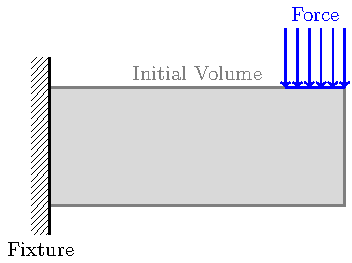
\includegraphics[scale=1]{Pictures/tikzCantilever/canti.pdf}
\end{center}
\caption{Boundary conditions for the test case "Cantilever".}
\label{fig:cantiBC}
\end{figure}
First this scenario is modelled in CAD (see \autoref{fig:cantiCAD}). After the optimization a lightweight structure is obtained (see \autoref{fig:cantiOPTIM}). One observes that in comparison to the original design topological changes have been introduces. The resulting NURBS surface is represented by $2202$ single NURBS patches and has a volume fraction of approximately $28\%$ compared to the initial volume.
\begin{figure}[H]
\begin{subfigure}[t]{.45\textwidth}
\begin{center}
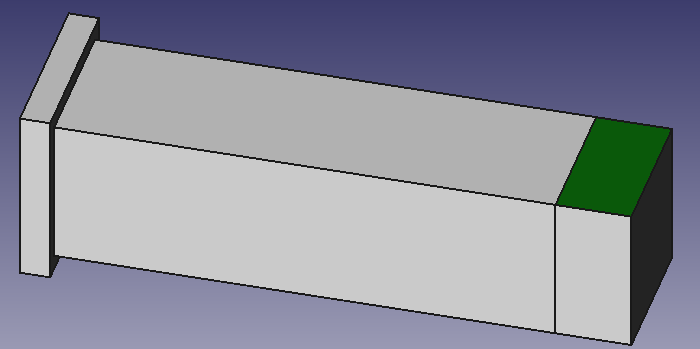
\includegraphics[width=.9\textwidth]{Pictures/Results/CantiIn.png}
\end{center}
\caption{CAD design}
\label{fig:cantiCAD}
\end{subfigure}
\begin{subfigure}[t]{.45\textwidth}
\begin{center}
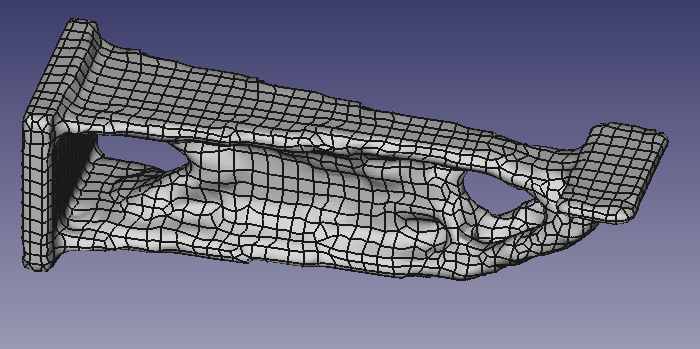
\includegraphics[width=.9\textwidth]{Pictures/Results/CantiOut.png}
\end{center}
\caption{Optimized structure}
\label{fig:cantiOPTIM}
\end{subfigure}
\caption{Test case "Cantilever"}
\end{figure}

\subsection{Bridge}
\label{ssec:bridge}
The second test scenario resembles a bridge, that is modelled through a volume resting on two supports and a plane - the intended driving plane - in the middle of the volume subjected to an area force (see \autoref{fig:bridgeBC}).
\begin{figure}[H]
\begin{center}
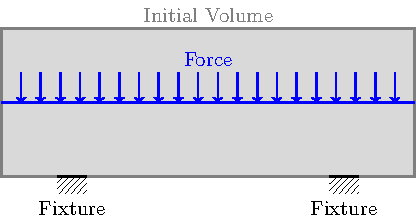
\includegraphics[scale=1]{Pictures/tikzBridge/bridge.pdf}
\end{center}
\caption{Boundary conditions for the test case "Bridge".}
\label{fig:bridgeBC}
\end{figure}
After modelling the bridge in CAD (see \autoref{fig:bridgeCAD}) and running the optimization algorithm, a structure is obtained, that resembles a bridge (see \autoref{fig:bridgeOPTIM}). The optimized structure is represented by $868$ NURBS patches and has a volume fraction of approximately $15\%$ of the initial volume.
\begin{figure}[H]
\begin{subfigure}[t]{.45\textwidth}
\begin{center}
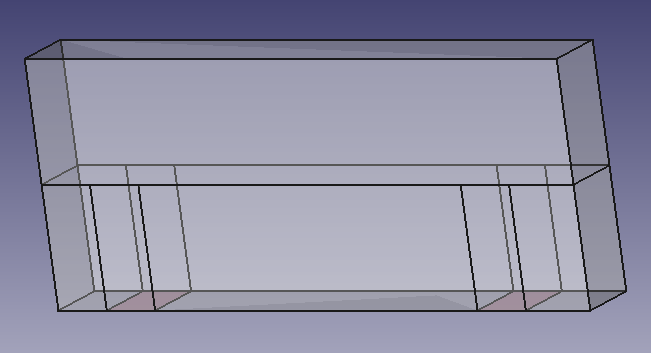
\includegraphics[width=.9\textwidth]{Pictures/Results/BridgeIn.png}
\end{center}
\caption{CAD design}
\label{fig:bridgeCAD}
\end{subfigure}
\begin{subfigure}[t]{.45\textwidth}
\begin{center}
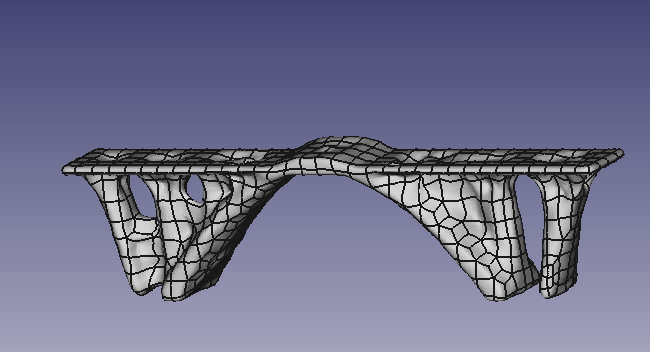
\includegraphics[width=.9\textwidth]{Pictures/Results/BridgeOut.png}
\end{center}
\caption{Optimized structure}
\label{fig:bridgeOPTIM}
\end{subfigure}
\caption{Test case "Bridge"}
\end{figure}

\subsection{GE Jet Engine Bracket}
\label{ssec:bracket}
On the contrary to the previous two tests, the final test case resembles a real application scenario. The load conditions and the initial volume originate from a topology optimization challenge proposed by General Electric in 2013 \cite{GEBracket}. The original goal of the challenge was the optimization of a jet engine bracket, that is subjected to four different load conditions and five different non-changing regions (see \autoref{fig:GEbracketBC}).
\begin{figure}[H]
\begin{center}
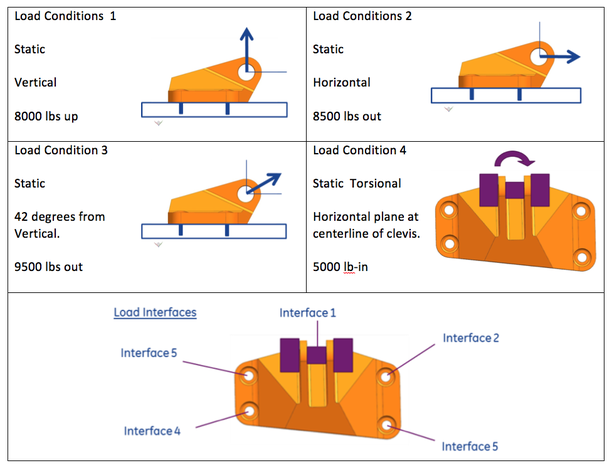
\includegraphics[scale = 0.4]{Pictures/GEbracket.png}
\end{center}
\caption{Boundary conditions and different load cases for test case "GE Bracket". Figure from \cite{GEBracket}.}
\label{fig:GEbracketBC}
\end{figure}
In the following an already optimized design from \cite{GEBracketTripon} was chosen, since the scale of the scenario was to big to be handled by ToPy. Therefore, the task for the last test case was only the reconstruction of the given geometry, in order to investigate the performance of the algorithm for real world applications. While the original design is described by $226$ faces, the reconstructed version took $3202$ NURBS patches. Additionally some topological features are lost in the region close to "Interface 1".
\enlargethispage{2cm}
\begin{figure}[H]
\begin{subfigure}[t]{.45\textwidth}
\begin{center}
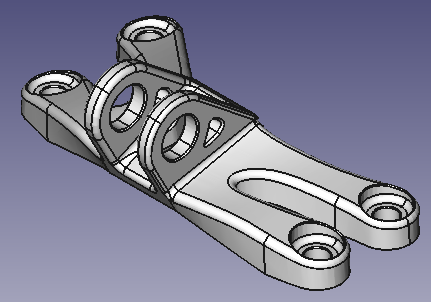
\includegraphics[width=.9\textwidth]{Pictures/Results/BracketIn.png}
\end{center}
\caption{CAD design. Initial geometry is already an optimized design from \cite{GEBracketTripon}.}
\label{fig:GEbracketCAD}
\end{subfigure}
\begin{subfigure}[t]{.45\textwidth}
\begin{center}
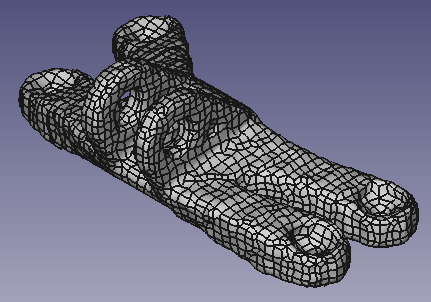
\includegraphics[width=.9\textwidth]{Pictures/Results/BracketOut.png}
\end{center}
\caption{Reconstructed structure}
\label{fig:GEbracketOPTIM}
\end{subfigure}
\caption{Test case "GE Bracket"}
\end{figure}

\section{User Experience}
\label{sec:uex}
From the user point of view CADO  is very simple. One doesn't have to know anything about the algorithms behind nor about the implementation details. Graphical User Interface (see \autoref{fig:mainWindowParameters}) allows the user to enter all the necessary information right a way, without keeping in mind the order of the parameters. Closed structure of the pipeline allows us to hide all the technical details from the user. However, user can still see on which stage the process is right now by looking at the progress bars, corresponding to the three major steps:
\begin{itemize}
\item Voxelization
\item Topology Optimimzation
\item Surface Fitting
\end{itemize}
Further information and the detailed description of the user interface can be found in the userguide (\textit{CADO\_UserGuide.pdf}).